% Integrated general architecture, reconciled with the current specification.
\section{Solution Architecture}
\label{sec:solution-architecture}

\subsection{System Context}
OliveTrack is proposed as a progressive web application (PWA), supported by a
central business API, relational persistence and private file storage. Phones and
tablets are the primary field devices; desktop access uses the same responsive
application across the supported desktop layout. The design aims to support quick field entry,
prepared offline continuity, explicit central validation and business isolation.

The private deployment serves one client business for Pepe's parents. A Technical
Administrator provisions its initial owner and workspace online. Invited Field
Managers continue their owner-issued invitation and account-verification flow.
The Farm Owner and invited Field Managers use individual accounts within the
owner's business workspace. Workers have business-specific records and may review
and sign documents on an authorised user's device; they do not need accounts.
The cooperative and laboratory supply information entered or attached by users.
Direct integration with those organisations is outside the current scope.
Email delivery is an external dependency for verification, invitations,
recovery and verified-email changes. The backend owns transactional sending under
\identifier{SEC-11}; provider/domain selection remains under \decisionref{Q-NFR-05}.

The approved working stack is React with TypeScript, Vite and Tailwind CSS for an
installable PWA, IndexedDB for protected prepared data/outbox, one modular
Node.js/NestJS backend and PostgreSQL. Shared TypeScript contracts and pure rules
support previews; the server remains authoritative. The end-to-end technical validation
under \decisionref{Q-ARCH-01} is still required. This description does not establish that a production
system, deployment or synchronisation mechanism has been implemented or verified.
The single-final-delivery model follows Section~\ref{sec:final-delivery}; the prior prototype's status and
presentation date are recorded in Section~\ref{sec:document-status}.

\begin{figure}[!htbp]\centering
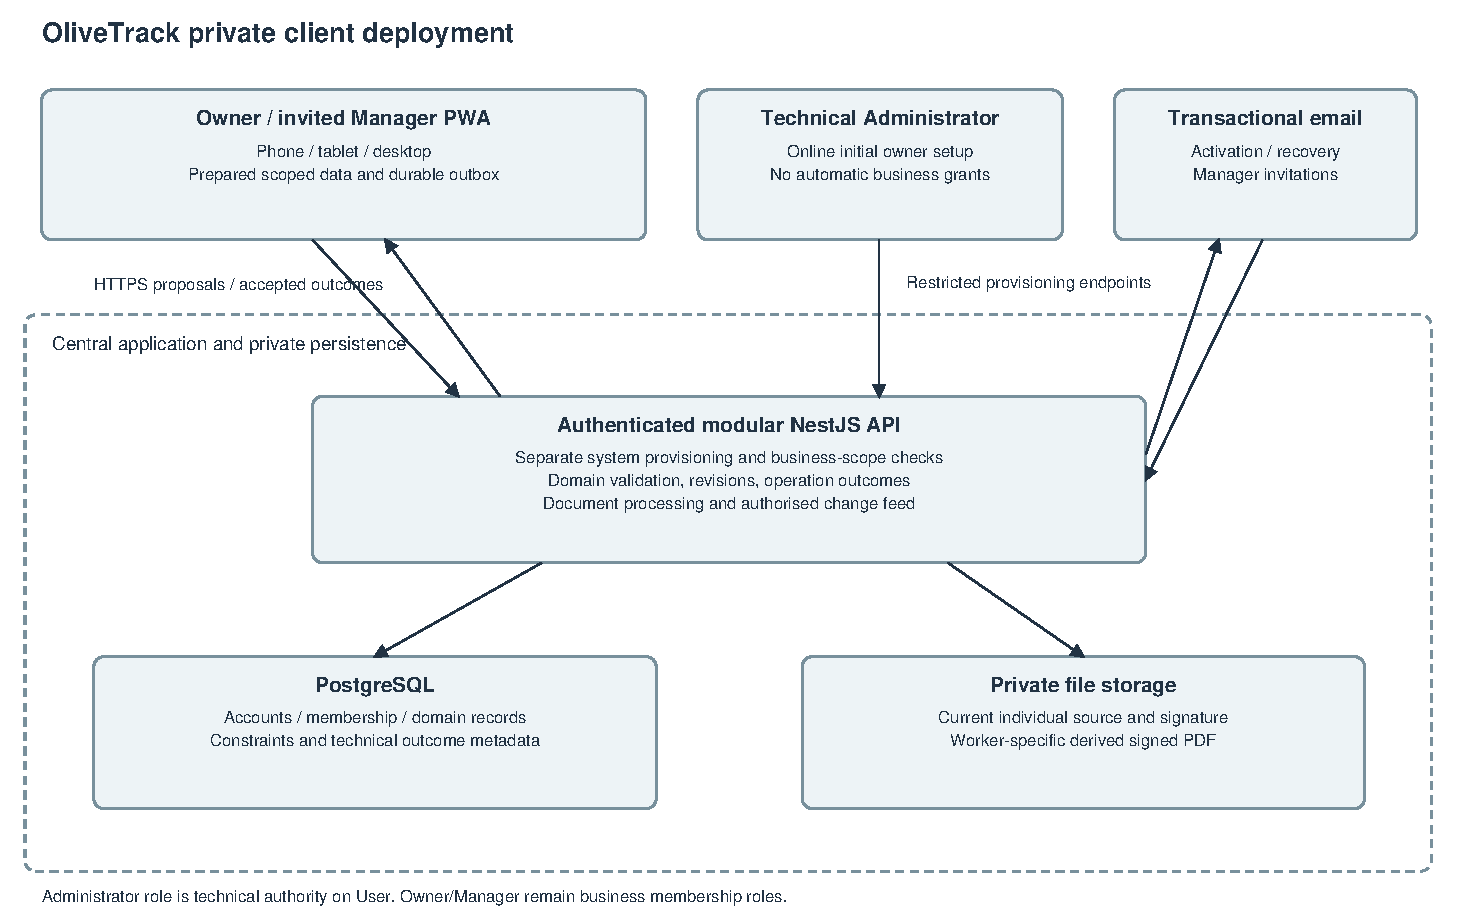
\includegraphics[width=0.98\linewidth]{solution-components-review.pdf}
\caption{Component responsibilities and separate technical/business authority. Restricted provisioning and scoped business endpoints use the same modular API. Device-local proposals and private central storage remain separate trust boundaries; no browser has direct database access.}
\label{fig:solution-components}
\end{figure}\FloatBarrier

\subsection{Components and Responsibilities}
\subsubsection{Client Application and Local Storage}
The React PWA uses Vite for builds and Tailwind CSS for responsive
presentation. A service worker prepares the application shell; IndexedDB holds
the authorised local dataset, file availability metadata and durable outbox.
Browser caching alone is not a business-operation queue. Save each supported
proposal and its outbox entry atomically before reporting local success.

Prepare only the required scope and permitted source versions/files. Include
insurance consultation and selected-version signing under their grants, rather
than excluding all contracts or insurance from offline use. Prepared financial
consultation, entry, correction and PDF output also follow their grants. Record
file readiness separately from structured-record acceptance. Preserve pending
dependencies through normal app closure and restart while browser storage remains
intact; clearing storage or losing a device can destroy exclusively local work.
Storage checks and warnings follow \identifier{AOC-05}.

The interface uses the business and synchronisation states in
Section~\ref{sec:sync-states}. A generic failure label must not obscure the
difference between transmission failure, rejection, conflict and an uncertain
server outcome. Normal field interaction remains simple, with recovery detail
shown when action is needed, as defined in Section~\ref{sec:offline-interaction}.
Browser-background execution is not assumed to be continuously available: retry
when execution and connectivity permit, and provide an explicit retry/review path.

\subsubsection{Identity and Delegated Access}
User identifies the account; WorkspaceMembership carries the contextual role and
AccessGrant carries permitted operations and owner-assigned responsibility scope.
Each owner has one business workspace. A real person working for different owners
may have separate Worker records; no global worker directory or cross-business
identity merge is introduced. The Owner role does not prove legal property title.

Technical account provisioning validates the separate administrator system role.
The administrator receives no operational grants automatically. Every protected
business API read, write, export and file request validates account, membership, operation and scope. Never trust a workspace identifier or role sent
by the browser. Preserve the reviewed manager defaults and mandatory scoped
insurance consultation in Section~\ref{sec:permission-defaults}; other document
and financial operations retain their independent grants. Property-based scope
includes parcels and current/future campaigns, permits multiple managers and
filters multi-property views to authorised contributions. Explicit worker
availability does not grant visibility of other-property work; see
\decisionref{Q-AA-02}.

Prepared offline authorisation expires 15 days after the latest successful online
permission validation. It is distinct from online-session expiry and 30-day
accepted-cache cleanup. Logout blocks local access while protecting recoverable
pending proposals; it does not indiscriminately erase the outbox. Offline devices
cannot receive immediate revocation or remote wiping. Central access checks,
reconnection and the local expiry gate enforce the applicable boundary. The
trusted-time, local protection and restricted owner-review mechanisms remain
subject to the existing security decisions.

\subsubsection{Business API and Domain Modules}
The Node.js/NestJS API is organised into cohesive modules in one backend
application. This modular structure does not require independently deployed
microservices. Module responsibilities follow the current data model:

{\compacttable
\begin{longtable}{L{0.27}L{0.73}}
\caption{Proposed backend modules.}\label{tab:backend-modules}\\
\toprule\rowcolor{TableHeader}
\textbf{Module} & \textbf{Responsibility}\\\midrule\endfirsthead
\toprule\rowcolor{TableHeader}
\textbf{Module} & \textbf{Responsibility}\\\midrule\endhead
\multicolumn{2}{r}{\footnotesize\itshape Continued on next page}\\\endfoot
\bottomrule\endlastfoot
Access and workspaces & Initial owner provisioning, activation/recovery, invitations, memberships and operation-specific grants.\\\midrule
Properties and campaigns & Properties, optional parcels, coverage, explicit execution start, closure, reopening and archival rules.\\\midrule
Workforce and work & Identified workers, capabilities, optional plans, daily attendance, actual assignments, periods, tasks and breaks.\\\midrule
Worker documents & Uploaded/generated source versions, one worker per document, templates, signatures, renditions and retention.\\\midrule
Harvest logistics & Delivery-associated transport, actual load origins, driver/vehicle references and weighing tickets.\\\midrule
Analyses and indicators & Delivery analyses, current ticket-reported amounts, assigned-weighted yield and scoped indicators/PDF summaries.\\\midrule
Synchronisation & Operation outcomes, revisions, ordered dependencies, authorised change feed and reviewed conflict/recovery paths.\\
\end{longtable}}

\subsubsection{Shared Rules and Central Persistence}
A shared TypeScript package provides types and pure validation/calculation
functions used by client and server. Local results are previews while acceptance
is pending. Shared code does not replace server authorisation, complete-data checks
or database integrity. The server recalculates and validates accepted changes.

PostgreSQL stores the model in Section~\ref{sec:data-architecture}. Use foreign keys, uniqueness,
checks, transactions and suitable cross-record enforcement. Same-workspace
references, actual-period non-overlap and exclusive accepted campaign execution
need more than ordinary independent row checks. Keep technical idempotency and
deletion metadata separate from permanent business field history.

Each delivery has at most one ticket and one analysis, and each ticket has one
current reported monetary value. A reported final amount replaces its provisional
predecessor; ordinary corrections retain current values. Store reported values
and units, with validated source metadata and independent printed processing
duration. KILOS ASIGNADOS supplies accepted assigned kg, total kg is separate and MEDIANERIA is the accepted percentage rather than laboratory yield; no assumed penalty tariff or repeated deduction is applied.
Calculate aggregates from eligible sources under Section~\ref{sec:calculation-rules}.
Weights, yields and monetary totals include only Delivered, non-cancelled
deliveries with the required inputs. Local arrival can update provisional local
indicators; central totals require accepted arrival and source records.

\subsubsection{Files, Generation and Signing}
Files are required architecture components. Keep them private in an object store
or equivalent protected service, with authorised access through the API or
short-lived scoped links. A private S3 bucket is a deployment candidate; document workflows do not depend
on selecting that provider. Validate each file request and keep
secrets and reusable privileged credentials out of the browser bundle.

Maintain immutable source identities/content hashes, document versions, per-worker
signature evidence and worker-specific derived signed PDFs. Capture the worker's
review and confirmation for the selected version; the operator's account identifies
the facilitator and does not replace the worker as signer. A later source version
needs its own signing event. Template generation under \identifier{UC-20} and
\identifier{FR-063} produces reviewed unsigned source versions; available templates
use the four supplied Spanish forms in Table~\ref{tab:source-forms}, preserving their wording under \decisionref{Q-DOC-01}. Decision-bearing forms add a typed choice
to worker/version evidence, committed atomically with signature acceptance and
rendered on the worker-specific PDF. Generation leaves the choice unselected. The workflow does not issue official identity
or work-permit evidence.


Retention follows \identifier{BR-026} and Section~\ref{sec:data-lifecycle}: keep
each current document source, signature and PDF until a complete replacement is accepted,
then delete the old graph for every category without inheritance or a history view.
Explicit ticket/analysis/value-attachment replacement also deletes the previous file
after success. Failed uploads preserve the current source/evidence. Coordinate this
with minimal deletion/idempotency metadata, private object storage and safe retries;
a database transaction alone does not atomically delete an object-store file.
The 10~MB PDF/JPG/JPEG/PNG policy applies to uploads. A captured mark and digest
do not certify legal identity; manual privacy/operational procedures remain separate
deployment preparation. The team implements/tests protection and recovery within
the agreed current-only and exact-source signing policies.

\subsection{Main Interaction Flows}
\begin{enumerate}
\item \textbf{Connected preparation.} Authenticate and validate permissions, then
prepare selected reference data, schedules and permitted files. Account/access,
property structure, campaign creation/coverage/closure/reopening, existing-worker
administration, source-version management and generation use connected workflows.
\item \textbf{Field entry.} Review and confirm a supported operation, durably save
its local proposal and dependencies, and show its actual save state. Prepared
explicit campaign starts and identified same-day worker creation are supported
offline exceptions; they do not make all administration available offline.
\item \textbf{Central acceptance.} Authenticate again as needed, check current
authority, operation identity, revision, dependencies and business rules, and commit
the outcome consistently. Reconcile the result without duplicate business effects.
\item \textbf{Review and completion.} Consult authorised incoming changes and
indicators, resolve conflicts explicitly and complete late source information.
Campaign closure/correction exceptions follow the use cases and rules, not an
append-only restriction on all business records.
\end{enumerate}

\subsection{Offline Operation and Synchronisation}
\label{sec:offline-sync}
\label{sec:offline-synchronisation}
The proposed protocol separates durable local proposals from centrally accepted
records. Prepared datasets and local/central storage responsibilities are described
in Section~\ref{sec:data-local-central}. Authentication limits, recovery mechanisms
require technical validation even where their behaviour and selected stack are approved.


\subsubsection{Local Proposals and Ordered Dependencies}

Each proposed operation is identified by a stable \texttt{operation\_id}, origin
User, Workspace, entity type and ID, and operation kind.
For validation, it also carries the payload, base revision for updates, dependency
IDs and client recording time. The local outbox uses the states in
Section~\ref{sec:sync-states}, with separate retry detail.
Client timestamps do not prove central acceptance or prior authorisation.
Use stable client-generated record identifiers for offline creation; the selected
UUID generation method must be consistent across devices and server.

The selected local store must persist each business proposal and its outbox entry
atomically before the application reports a successful local save. Show local confirmation separately from acceptance.
Submit dependencies first: a delivery before its ticket, a version before signing,
and accepted metadata/file readiness before dependent references. Basic worker creation and explicit campaign start are supported exceptions.
Queue a worker before attendance, assignments and driver references. Individual
document creation/source acceptance is online and requires that worker first;
prepare that accepted source before offline signing. Queue campaign start before dependent
execution records. Administration of existing profiles and property creation remain online.


Use one stable client-generated Worker UUID and operation UUID through local
creation and acceptance. Pending references must not be replaced by an unrelated
identity if a duplicate warning appears. Resolve an existing/new identity only
through an explicit reviewed procedure that preserves work, document associations
and files; no automatic merging or cross-business lookup is introduced.

An explicit start proposes Planned to In progress. The server validates authority,
actual dates and competing execution atomically before accepting dependent records.
Concurrent offline starts on one area cannot both become accepted; keep the rejected
or conflicting start and its dependencies recoverable. A device timestamp is not
an authoritative proof of an exclusive reservation.


\subsubsection{Central Acceptance, Conflicts and Incoming Changes}

For each request: authenticate the account, determine the operation workspace,
validate current authority, check operation identity and compare its fingerprint,
then validate base revision and domain invariants in a transaction. A reused ID
with different content is not the same retry. Commit the business change and its
idempotency outcome consistently, and return affected identities/revisions.
An outcome ledger stores minimal replay status, not a permanent full copy of every
old business row. Retain minimal operation outcomes for 90 days after processing
and change/deletion-feed markers for 90 days. Support the preceding client/payload
version for 30 days after a release. Server-issued validity context must route
stale requests to refresh/reviewed recovery; missing expired metadata never proves
that a request is new. Validate safeguards against duplication and resurrection.

An uncertain transmission triggers operation-status checking or safe retry.
Never assume that timeout means no central change. A stale base revision produces
a conflict, not Last Write Wins. Authorised users compare accepted values and the
proposal, then keep accepted data or resubmit a reviewed correction for validation.


The server supplies only changes the account may receive, using a proposed durable
cursor. Apply business changes, deletion markers and cursor advancement consistently.
A deletion marker is a technical synchronisation fact, not a field-change history.
After access reduction, the client removes inaccessible prepared data without
submitting it through another account. Beyond the valid change-retention window,
refresh authorised data rather than silently missing old deletions.

Track attachment upload separately from structured-record acceptance. Keep failed
uploads recoverable and do not expose an unavailable object as stored. A replacement
version becomes current only once its source is available. Offline retention cleanup
must not revive deleted versions when a pending signature reconnects.


\subsubsection{Access Expiry, Logout and Recovery}

Logout blocks local access but preserves recoverable pending work in account-isolated
protected storage. Renewed authentication is required for normal recovery.
Revocation is enforced online and on reconnection or offline expiry; no instantaneous
remote wipe of disconnected devices is asserted.

Existing pending manager proposals may enter a restricted Owner-review workflow
without restoring manager workspace access. Preserve origin and reviewer, and run
all campaign, date, revision and dependency checks on acceptance. Owner acceptance
supplies new explicit authority; client timestamps cannot establish pre-revocation
creation. The origin account authenticates only for restricted submission, without
normal workspace access. Concrete protected transport/quarantine/expiry remains
a verification task. Signing-source eligibility cannot be overridden by approval.


Enforce \hyperref[br:002]{\identifier{BR-002}} through a local gate storing the last successful
online permission-validation instant and expiry. Cached use and cleanup cannot
renew it. Protect this context against simple clock rollback; the trusted-time
mechanism remains a security design decision. Expiry blocks consultation/new
operations but preserves protected recoverable proposals until online revalidation.
It does not deliver server changes; the authorised change feed does that.

The routine presentation follows Section~\ref{sec:offline-interaction}. A simple
status does not replace durable outbox storage, dependency checks or idempotency.
Local protection and expiry follow \identifier{PRV-03}/\identifier{AOC-02}; the final mechanism remains
under \decisionref{Q-DOC-07}. Warning/retry timing and concrete local security
mechanisms remain pending; approved session/backup/recovery/availability targets
are specified by their owning NFRs. \identifier{REL-08} and \decisionref{Q-NFR-06} govern restricted
owner-review recovery, not a normal submission bypass.

\subsubsection{Local Indicators and Operation Boundaries}

Use the last accepted available baseline plus identifiable local proposals: create
once, replace on update and remove the previous contribution on local removal.
Label affected values provisional and disclose missing/partial scope and last sync.
Apply the same Delivered, non-cancelled eligibility to all delivery-based totals.
A local arrival confirmation enables eligible contributions in the provisional
view; pre-arrival source data remains in detail awaiting receipt confirmation.
Central totals use only server-accepted arrival confirmations and source values.
Rejected proposals do not remain part of accepted totals. Never imply knowledge of
other-device changes since last synchronisation. Offline PDF may include authorised prepared financial information and records generation time, scope, freshness, missing information and pending data. Financial source provisional/final status is separate from synchronisation status.



The outbox accepts only the operations supported in
Section~\ref{sec:non-functional-requirements}; connected administration and source
generation use online endpoints. Prepared datasets/file manifests enforce the
operation and complete-file restrictions in Section~\ref{sec:conceptual-files}.
Coordinate source, evidence and rendition cleanup with protected signing operations;
exclusively local signatures may require \decisionref{Q-DOC-04} resolution.
Cancellation remains a domain update in the change feed, rather than a deletion
marker, preserving dependencies while removing indicator contributions.


\subsection{Deployment and Operation}
\subsubsection{Proposed Hosting Arrangement}
Separate static PWA delivery, the application API, PostgreSQL and private file
storage. The contribution suggests AWS in an EU region: S3/CloudFront for the
application, an evaluated container service for the API,
RDS for PostgreSQL, private S3 files, Secrets Manager and CloudWatch.
This is an example topology under \decisionref{Q-ARCH-02}; it is not a procurement
decision, a free-tier guarantee or evidence of operational availability. Evaluate
an academic/managed alternative if necessary without weakening access, integrity
or document controls. Application-managed authentication is selected; choose the transactional email provider separately.

The EU-region preference does not itself demonstrate privacy compliance. Review
processing locations, provider roles, transfers and costs under
\decisionref{Q-NFR-03} and \decisionref{Q-ARCH-02}. Use synthetic or appropriately
anonymised demonstration data until the processing basis for real personal data
has been established. Configure encrypted transport/storage, least-privilege
service access and secret management against Section~\ref{sec:nfr-security}.

\subsubsection{Code Organisation and Delivery}
The proposed monorepo separates client, server and shared contracts/rules.
Pin dependencies and review generated or contributed code under the same standards.
GitHub Actions can run build, lint, unit/integration checks and migration validation
before merge/deployment. Docker is proposed for reproducible server packaging;
choose one infrastructure-as-code approach, such as Terraform or AWS CDK, only
if it fits the team's capacity. These engineering mechanisms remain planned.

Changes to local schemas, service workers and API payloads must preserve pending
work and account for older cached clients. Store the client/payload version with
sync requests and reject unsupported formats recoverably. Do not force an update
that clears queued work. Use reviewed migration and rollback procedures; an old
application release is usable only with a compatible schema and payload contract.
The approved 30-day preceding-client compatibility policy is specified in \identifier{REL-07} and
\decisionref{Q-NFR-02}.

\subsubsection{Operational Verification}
Assign monitoring, incident, backup and restore responsibilities before operational
use. Managed services do not remove application-level configuration or restore
testing. Approved availability, daily/14-day backup, RPO/RTO and performance
targets are specified in the owning NFRs; do not create independent architecture
targets or imply they have been measured. Central backups cannot recover changes that never left a lost device.
Security audit events have a separate purpose and retention policy from business
correction history.

Measure rendering, durable local saving, central acknowledgement, structured replay
and file transfer separately. Synthetic probes must not expose worker data or
disable supported offline entry. Validate phone/tablet usability and recovery
feedback under Section~\ref{sec:nfr-usability} and \identifier{AOC-06}. Test
retries, concurrent edits, offline starts/new workers, storage interruption and
source/signature retention before claiming the corresponding behaviour works.
Section~\ref{sec:risk-management} records the project risks affecting delivery.

\subsection{Architecture Decisions and Remaining Validation}
The reviewed specification already separates planned and actual work, local
confirmation and server acceptance, source files and signed renditions, and
business corrections and technical replay metadata. Stable identities, idempotent
effects and optimistic revision checks with explicit conflict review are retained.
Last Write Wins is not an alternative conflict policy in this baseline.

\decisionref{Q-ARCH-01} records the selected stack and the outstanding tested vertical slice; \decisionref{Q-ARCH-02} covers hosting, service selection,
costs and operating ownership. These do not reopen the included manager, prepared
document/signing flows, authorised offline finance or one-ticket/one-analysis rules.
Property scope, owner-authorised recovery and metadata lifetimes are decided.
Concrete local encryption/key handling, trusted-time enforcement, safe expired-context
recovery and legal/operational signing suitability retain the specific validations
in Section~\ref{sec:uc-open-decisions}.
Implementation and verification target the single final delivery under
\decisionref{Q-SCOPE-01}; internal technical slices are development steps.

\paragraph{Rationale and trade-offs.}
The following decisions explain the proposal's main quality drivers. They record
design reasoning, not comparative benchmark results or final procurement approval.
{\compacttable
\begin{longtable}{L{0.23}L{0.45}L{0.32}}
\caption{Architecture rationale, trade-offs and validation needs.}\label{tab:architecture-rationale}\\
\toprule\rowcolor{TableHeader}
\textbf{Proposed choice} & \textbf{Reason / requirement driver} & \textbf{Trade-off / validation}\\\midrule\endfirsthead
\toprule\rowcolor{TableHeader}
\textbf{Proposed choice} & \textbf{Reason / requirement driver} & \textbf{Trade-off / validation}\\\midrule\endhead
\multicolumn{3}{r}{\footnotesize\itshape Continued on next page}\\\endfoot
\bottomrule\endlastfoot
Responsive PWA with IndexedDB outbox & One phone/tablet interface and prepared field continuity; atomic local proposals support \identifier{FR-034} and \identifier{AOC-03}. & Browser storage and execution limits require device tests; protection and trusted time remain under \decisionref{Q-DOC-07}.\\\midrule
Modular TypeScript API and shared pure rules & Modules follow domain responsibilities; shared previews reduce divergent calculations, while the server enforces \identifier{REL-03}. & Shared code does not supply authority or concurrency guarantees. Validate the selected stack through the technical slice under \decisionref{Q-ARCH-01}.\\\midrule
PostgreSQL transactional acceptance & Relationships, uniqueness and serialised validation support single tickets/analyses, attendance and exclusive execution. & Cross-record checks need a tested transaction/locking design, not only independent row checks.\\\midrule
Stable operations and optimistic revisions & Safe retries and explicit conflict review preserve \identifier{REL-01}/\identifier{REL-02} without silent last-write-wins. & Adds dependency and recovery work; expired-context safeguards and owner-authorised recovery remain verification tasks.\\\midrule
Private object storage plus relational metadata & Keeps source files, signature evidence and derived PDFs distinct under \identifier{SEC-08} and \identifier{BR-026}. & Database/file readiness and cleanup need recoverable coordination; provider/cost and retention are separate decisions.\\\midrule
Managed hosting candidate & Separates application delivery, API, database and files while supporting configurable backup/monitoring. & Compare an affordable deployment against the agreed NFRs; AWS is an option under \decisionref{Q-ARCH-02}, not a free or approved service guarantee.\\
\end{longtable}}


\paragraph{Required technical slice.}
Authenticate and prepare an authorised campaign/worker; durably save field work
offline; close/reopen the PWA and verify persistence; reconnect and accept centrally;
retry the same operation without duplicate effects; then create a competing revision
and verify explicit conflict recovery. Include stale-context recovery, local
encryption/key lifecycle and fail-closed expiry boundary checks before claiming
the corresponding architecture is feasible on the supported devices.

\paragraph{Supplied skeleton and implementation gap, 24 November.}
The supplied archive contains npm workspaces, NestJS/Prisma, PostgreSQL Compose,
React/Vite/Tailwind PWA configuration and a Task-only Dexie/outbox example. Its
schemas and migrations model Task/AppliedMutation, its manifest identifies a task
application and its example sync chooses newer client timestamps. It provides
starting files to adapt and verify under the task catalogue. Domain contracts,
scoped authentication/provisioning, schema migrations and explicit revision conflict
handling still need implementation. Replace the example LWW path before accepting
agricultural mutations under this baseline. Validate source readiness, permissions,
retained pending work and supported PWA update behaviour through the technical slice.
